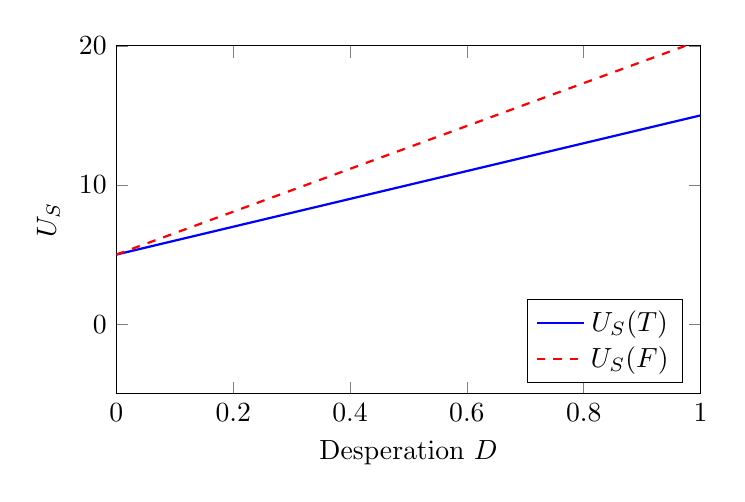
\begin{tikzpicture}
\begin{axis}[
    width=9cm,
    height=6cm,
    xlabel={Desperation $D$},
    ylabel={$U_S$},
    xmin=0, xmax=1,
    ymin=-5, ymax=20,
    legend style={at={(0.97,0.03)},anchor=south east},
    domain=0:1,
    samples=100
]
% Example parameterization:
% alpha(D) = 1 + 2D, beta(D) = 1 - 0.7D
% Truth: R_T = 5, C_T = 0
% Fabrication: E[R_F]=7, E[C_F]=2
\addplot[blue, thick] {(1 + 2*x)*5};
\addlegendentry{$U_S(T)$}

\addplot[red, thick, dashed] {(1 + 2*x)*7 - (1 - 0.7*x)*2};
\addlegendentry{$U_S(F)$}

\end{axis}
\end{tikzpicture}
